\documentclass{beamer}

\usepackage{hyperref}
\usepackage{tikz}

%\setbeameroption{show only notes}
% \usetheme{material}

\usetheme[progressbar=frametitle, numbering=fraction]{metropolis}
% \usetheme[sectionpage=none,progressbar=frametitle, numbering=fraction]{metropolis}  

\title{%
  \textbf{Question Answering and \\Lifelong Learning} \\%
  {\small Programme: Intelligent Systems}
}
\author{%
  Guillermo Echegoyen\\%
  {\color{gray}\footnotesize Advised by: \\$\-$ Anselmo Pe\~nas \\$\-$ Alvaro Rodrigo}\\%
}

% \institute{UNED ETS. Inform\'atica}
\date{}

\titlegraphic{%
  \flushright
\includegraphics[width=2cm,height=2cm]{logo.png}
}

\addtobeamertemplate{frametitle}{}{%
  \begin{tikzpicture}[remember picture,overlay]
    \node[anchor=north east,yshift=2pt] at (current page.north east) {
\includegraphics[height=0.8cm]{logo}};
  \end{tikzpicture}
}

\setbeamercolor{frametitle}{fg=brown,bg=brown!20}
\setbeamertemplate{page number in head/foot}{}
\setbeamertemplate{frame footer}{Doctoral Symposium, June 2020}

\begin{document}
\maketitle

\begin{frame}{Table of contents}
  \setbeamertemplate{section in toc}[sections numbered]
  \tableofcontents[hideallsubsections]
\end{frame}

\section{Who am I}
\begin{frame}{Who am I}
  \begin{columns}[T,onlytextwidth]
    \column{0.45\textwidth}
    \begin{alertblock}{Background}
      \begin{itemize}
        \item Software Engineering
        \item AI Master
      \end{itemize}
    \end{alertblock}
    \column{0.45\textwidth}
    \begin{alertblock}{Where to find me}
      \begin{itemize}
        \item \href{https://geblanco.github.io}{Resum\'e}
        \item \href{https://scholar.google.es/citations?user=5XnvPusAAAAJ&hl=en}{Google Scholar}
      \end{itemize}
    \end{alertblock}
  \end{columns}
  \begin{alertblock}{Currently}
    \begin{itemize}
      \item International project LIHLITH-KIQA (PI: Anselmo Pe\"nas). Question Answering that evolve over time.
      \item First year PhD in Lifelong Learning Question Answering.
    \end{itemize}
  \end{alertblock}
\end{frame}

\section{Introduction}
\begin{frame}{Introduction}
  \alert{\Large Frame: LIHLITH project} \par
  LIHLITH-KIQA, IP: Anselmo Pe\~nas
  International coordinator: Eneko Agirre

  European funded project. PI: by Eneko Agirre. \par

  \textit{Learning to Interact with Humans by \\ Lifelong Interaction with Humans}

  \begin{itemize}
    \item Develop Question Answering and Dialogue Systems
    \item Enable them to evolve over time.
  \end{itemize}
\end{frame}

\begin{frame}{Introduction: Question Answering}
  % \metroset{block=fill}
  \begin{block}{Question Answering}
    \vspace{0.2cm}
    \textit{Systems that automatically answer questions posed by humans in a natural language} \\
    \begin{itemize}
      \item Open world assumption
      \item Closed world assumption
    \end{itemize}
    Applications:
    \begin{itemize}
      \item Question Answering Systems are everywhere, from personal assistants to chatbots and IT ticket management.
    \end{itemize}
  \end{block}
\end{frame}

\note[itemize]{%
  \item Open world assumption: Virtually, all resources can be used to retrieve the answer
  \item Closed world assumption: Closed set of resources to answer the posed question. Such as KG, a set of documents, a DB
}

\begin{frame}{Introduction: Lifelong Learning}
  % \metroset{block=fill}
  \begin{block}{Lifelong Learning}
    \vspace{0.2cm}
    \textit{Adapt previous knowledge to solve new, unseen problems.} \par

    Can be combined with many algorithms and different forms of learning:
    \begin{itemize}
      \item Neural networks
      \item Topic modeling
      \item Information Extraction
      \item Reinforcement Learning
    \end{itemize}
  \end{block}
\end{frame}

\section{Research Plan}
\begin{frame}{Research Plan}
  \begin{alertblock}{Objectives}
    \begin{itemize}
      \item Develop systems capable of detecting knowledge gaps
      \item Develop strategies to fill these gaps
      \item Enable QA systems to evolve over time
    \end{itemize}
  \end{alertblock}
  \begin{alertblock}{Research Questions}
    \begin{itemize}
      \item How to detect unanswerable questions given the available knowledge
      \item How to incorporate new knowledge with previous one
      \item How to asses systems effectiveness
        %talk about transfer Learning
    \end{itemize}
  \end{alertblock}
\end{frame}

\note[itemize]{%
  \item Information evolve over time (dates, dead) there is a need to evolve over time.
}

% internship?
\begin{frame}{Research Plan}
  \metroset{block=fill}
  \begin{alertblock}{1rst Year}
    \begin{itemize}
      \item Study state-of-the-art
      \item Gather evaluation collections
      \item Propose QA-LL system
      \item Propose method to develop evaluation collections
    \end{itemize}
  \end{alertblock}

  \begin{alertblock}{2nd Year}
    \begin{itemize}
      \item Develop collections for LL QA
      \item Evaluation and analysis of results
      \item Improvements from results
      \item Detect new challanges
    \end{itemize}
  \end{alertblock}
\end{frame}

\begin{frame}{Research Plan}
  \metroset{block=fill}
  \begin{alertblock}{3rd Year}
    \begin{itemize}
      \item Development of QA-LL System
      \item Evaluation and analysis of results
      \item Final draft with implemented system
    \end{itemize}
  \end{alertblock}

  \begin{alertblock}{4rd Year}
    \begin{itemize}
      \item Evaluation and final touches
      \item Write thesis
    \end{itemize}
  \end{alertblock}
\end{frame}

\section{Outcomes}
\begin{frame}{First Year Outcomes}
  \alert{\Large Publications (older to newer):}
  \begin{itemize}
    \item QA-LL task proposal: \cite{penas2019continuous}
    \item First evaluation collection: \cite{veron2020cooking}
    \item Survey on dialogue systems: \cite{deriu2019survey}
    \item Cross-lingual models: \cite{echegoyen2020crosslingual}
    \item Lifelong Learning Transformers (work in progess)
  \end{itemize}
\end{frame}

\begin{frame}{First Year Outcomes}
  \alert{\Large Question Answering-Lifelong Learning task proposal} \par

  Given a KG, and an external resource such as a text collection in the same domain:
  \begin{enumerate}
    \item Decide whether a user utterance in Natural Language can be mapped or not into the KG and, if this is the case
    \item Determine through which ones of the following ways the system must find a strategy to enrich the knowledge graph
  \end{enumerate}
  \begin{block}{Outputs}
    \item Shared task
  \end{block}
\end{frame}

\note[itemize]{%
  \item Work with the whole consortium
  \begin{itemize}
    \item Declare a new class (or object type). 
    \item Add a new instance of a class.
    \item Declare a new relation.
    \item Add a new triple to the KG.
  \end{itemize}
}

\begin{frame}{First Year Outcomes}
  \alert{\Large First evaluation collection:} \par

  \begin{itemize}
    \item Extract information from \href{https://en.wikibooks.org/wiki/Cookbook:Table_of_Contents}{Wikimedia Cookbook}.
    \item Organize and structure information as Knowledge Graph.
    \item Manually create both answerable and unanswerable questions from the KG.
    \item Manually annotate questions and answers.
  \end{itemize}

  \begin{block}{Outputs}
    \begin{itemize}
      \item Cooking Domain Knowledge graph
      \item Cooking Domain Question Answering dataset
    \end{itemize}
  \end{block}
\end{frame}

\note[itemize]{%
  \item Work with LIMSI (France)
}

\begin{frame}{First Year Outcomes}
  \alert{\Large Survey on Dialogue Systems} \par

  Study the state-of-the-art in:
  \begin{itemize}
    \item Task Oriented Dialogue System
    \item Conversational Dialogue Systems
    \item Question Answering Dialogue Systems
    \item Evaluation Datasets and Challenges
  \end{itemize}
\end{frame}

\note[itemize]{%
  \item Work with ZHAW (Switzerland) and the rest of the consortium
}

\begin{frame}{First Year Outcomes}
  \alert{\Large Cross Lingual Models} \par

  \alert{Goal:} Train a model in a language and transfer learning to another one (and another task).
  % Results table
\begin{center}
\resizebox{8cm}{!}{%
\begin{tabular}{l|c|c|c|c}
  \hline
  Dataset             & BERT     & MultiBERT        & Random   & Longest  \\ \hline
  RACE Mid            &  0.5265  & \textbf{0.6114}  & 0.2500   & 0.3078   \\
  RACE High           &  0.4774  & \textbf{0.5031}  & 0.2500   & 0.3059   \\
  RACE All            &  0.4917  & \textbf{0.5347}  & 0.2500   & 0.3059   \\ \hline
  EE English          &  0.4921  & \textbf{0.4974}  & 0.2500   & 0.2304   \\
  EE Spanish          &  0.3665  & \textbf{0.4503}  & 0.2500   & 0.2932   \\
  EE Italian          &  0.2880  & \textbf{0.4293}  & 0.2500   & 0.2775   \\
  EE French           &  0.3037  & \textbf{0.4346}  & 0.2500   & 0.2565   \\
  EE Russian          &  0.2618  & \textbf{0.3403}  & 0.2500   & 0.2723   \\
  EE German**           &  0.3708  & \textbf{0.4494}  & 0.2500   & 0.2584   \\ \hline
\end{tabular}
}
\end{center}

\end{frame}

\note[itemize]{%
  \item Not aimed to break SOTA, just a poc.
  \item No hyper-parameter tuning applied
}

\begin{frame}{First Year: Outcomes}
  \alert{\Large Lifelong Learning Transformers} \par

  \alert{Goal:} Reuse knowledge from previous tasks to boost performance of a new one while preserving effectiveness.
  
  \alert{ToDo}
\end{frame}

\note[itemize]{%
}

\section{Conclusions}
\begin{frame}{First Year Conclusions}
  \begin{alertblock}{Experimentation is hard:}
    \begin{itemize}
      \item Money for value
      \item Interpretability is difficult
      \item Catastrophic forgetting is hard to overcome
      \item We are far from real world QA systems
      \item Ideal laboratory settings are far from real world use cases
    \end{itemize}
  \end{alertblock}
\end{frame}

\note[itemize]{%
  \item Deep Learning aims for a number (accuracy). 
  \item Deployed systems face many more problems and inconsistencies than laboratory environments.
}

\section{Related Challenges}
\begin{frame}{Related Challenges}
  \alert{\Large Literature grows quickly}
  \begin{center}
    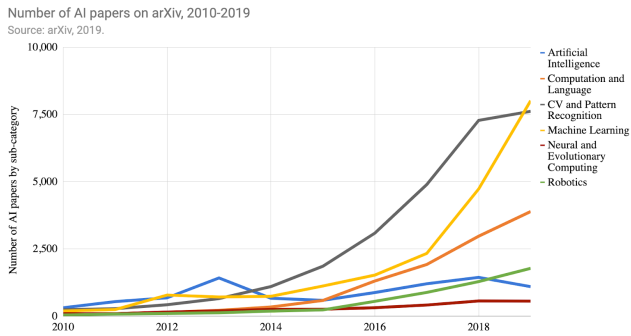
\includegraphics[width=0.9\textwidth]{./figures/ai_papers_arxiv_alpha.png}
  \end{center}
  \begin{flushright}
    {\tiny Artificial Intelligence Index Report 2019, Stanford University}
  \end{flushright}
\end{frame}

\begin{frame}{Related Challenges}
  \alert{\Large Trend towards Deep Learning}
  \begin{itemize}
    \item Large code base
    \item Programming GPUs
    \item Experiments are costly
    \item Cloud computing
    \item Results interpretation not always clear
  \end{itemize}
\end{frame}

\note[itemize]{%
  \item Many libraries
  \item Lots of algorithms
  \item AWS, GCP
}

% outro: ToDo := Add cool quote
\begin{frame}
  \begin{center}
    \Huge Thank you! \\
    \huge Questions? \\
    \Large Guillermo Echegoyen
  \end{center}
\end{frame}

\begin{frame}[allowframebreaks]{References}
  \bibliography{library}
  \bibliographystyle{abbrv}
\end{frame}

\end{document}
